\section{Big Data Analysis}

Big data analytics is where advanced analytic techniques operate on big data sets. Hence, big data
analytics is really about two things — \textit{big data} and \textit{analytics}.



\subsection{Big Data}

As the name suggests, big data is a large amount of data. There are other important attributes of big data. These are:  data variety and data velocity.

Thus we can define big data using 3 V's: \textit{volume}, \textit{variety}, and \textit{velocity} as showin in figure \ref*{bigData}.

\begin{figure}[h]
    \centering
    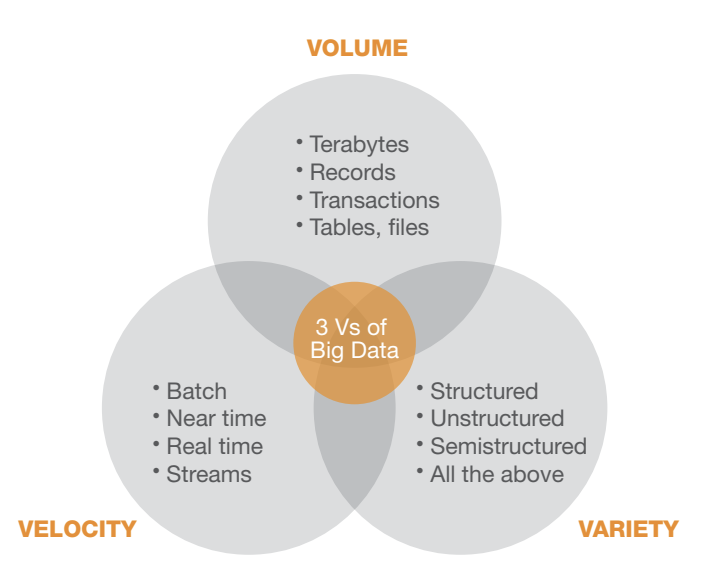
\includegraphics[width=0.5\textwidth]{images/big_data.png}
    \caption{Big Data: 3 V's \autocite{3vbigdata}}
    \label{bigData}
\end{figure}

Beyond these three V's, Big Data is also about how complicated the computing
problem is. Given the number of variables and number of data points for analysing the maritime shipping data. It is a very complicated problem.
Thus, in addition to the three V's identified by IBM, it would also be necessary to take complexity into account as shown in figure \ref*{bigDataComplex} \autocite{pence2014big}.

\begin{figure}[h]
    \centering
    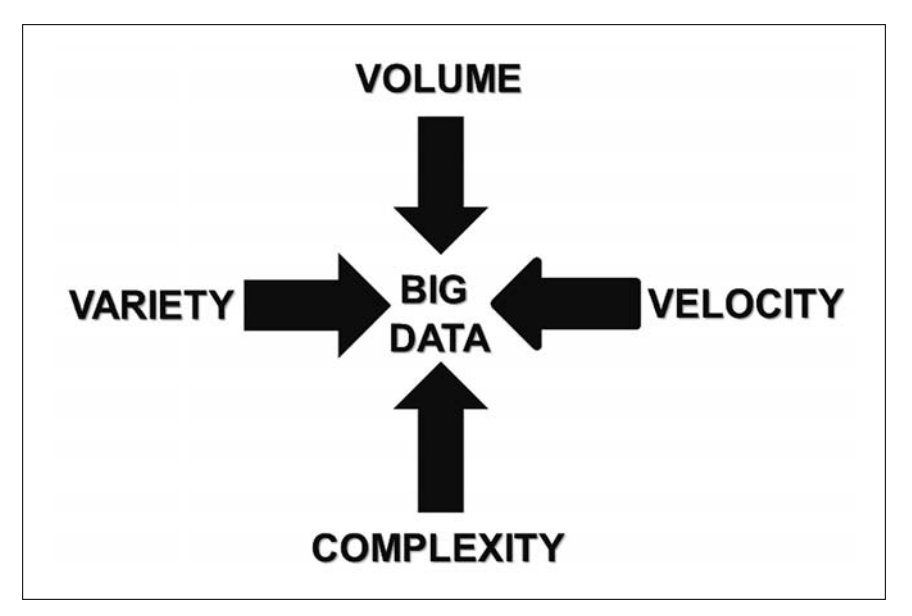
\includegraphics[width=0.5\textwidth]{images/big_data_complex.png}
    \caption{Big Data: Beyong 3 V's - volume, velocity,
        variety, and complexity}
    \label{bigDataComplex}
\end{figure}


\subsection{What is Big Data Analytics?}

Big data analytics is the process of examining large and varied data sets to uncover hidden patterns, unknown correlations, market trends, customer preferences and other useful information that can help organizations make more-informed business decisions.